\documentclass{beamer}
\usepackage{beamerthemeCambridgeUS}
\usepackage{color}  % for \textcolor{red}{blah}
\usepackage{graphicx}
\usepackage{subfigure}
\usepackage{multicol}
\usepackage{verbatim} % for \begin{comment}


\newenvironment{packed_enum}{
\begin{enumerate}
  \setlength{\itemsep}{1pt}
  \setlength{\parskip}{0pt}
  \setlength{\parsep}{0pt}
}{\end{enumerate}}

\newenvironment{packed_item}{
\begin{itemize}
  \setlength{\itemsep}{1pt}
  \setlength{\parskip}{0pt}
  \setlength{\parsep}{0pt}
}{\end{itemize}}

\usetheme{CambridgeUS}

\title{Discrete Mathematics}
\author[Geoffrey Buhl]{Geoffrey Buhl \\ \texttt{geoffrey.buhl@csuci.edu}}
\institute[CSUCI]{California State University Channel Islands}
\date{week 2 class 2}

\def \vec{{\rm vec}}
\newtheorem{conjecture}[theorem]{Conjecture}
\newtheorem{explanation}[theorem]{Explanation}


\begin{document}

%\frame{\titlepage}

%\section[Outline]{}
%\frame{\tableofcontents}

\section{Week 2}
\frame
{
  \frametitle{Unordered Selections}

Class Session Goals:
\begin{packed_enum}
\item Introduce Notation for Unordered selections and derive a formula
\item Present the Idea of a Combinatorial Proof
\item Work on applying the multiplication principle
\item Present connection of 'Choose' numbers and Binomial coefficents
\end{packed_enum}

}


\frame
{
  \frametitle{Order and Repetition}

How many ways are the to make $k$ choices from a list of $n$ possibilities? In order to make this a question that we can answer, we must answer the following two fundamental yes/no questions of Chapter 1. \vfill

{\bf Repetition} -  Are we able to repeat choices?  \vfill
{\bf Order} -Does the order in which we make the choices matter?   \vfill

For a given counting question, different answers are possible.  Goal of this chapter to create general formulas for each of the four situations.

}

\frame
{
  \frametitle{Some Answers}

{\bf Order Matters, Repetition not allowed}:The number of ways to make $k$ choices from $n$ where repetition is not allowed and order matters is $n \cdot (n-1) \cdot (n-2) \cdot (n-3) \cdots (n-k+1)=\frac{n!}{(n-k)!}$.\vfill


{\bf Order Matters, Repetition Allowed}:The number of ways to make $k$ choices from $n$ where repetition is allowed and order matters is $n^k$. \vfill

{\bf Todays question}:  How many ways are the to make $k$ choices from $n$ possibilities where repetition is not allowed and order does not matter?


}

\frame
{
  \frametitle{Binomial Coefficients}

Give the answer a name:
Let $\binom{n}{k}$ be the number of ways to make $k$ choices from $n$ objects where order does not matter and repetition is not allowed. Sometimes books use the notation $C(n,k)$ for this.
\vfill
Some Examples\\
$\binom{n}{1}=\pause n$\\ \vfill
$\binom{n}{n}=\pause 1$\\ \vfill
$\binom{n}{0}=\pause 1$\\ \vfill
$\binom{n}{2}=\pause \frac{n(n-1)}{2}$
\vfill
Our goal is general formula for $\binom{n}{k}$
}


\frame
{
  \frametitle{Activity}

Down Right paths on an $n \times n$ grid.

\begin{figure}[h]
  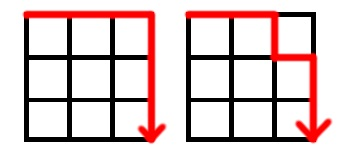
\includegraphics[scale=.50]{paths}

   \caption{Two down-right paths on a $3 \times 3$ grid.}
\end{figure}  

}
\begin{comment}

\frame
{
  \frametitle{Answers}

\begin{table}[htp]
%\caption{default}
\begin{center}
\begin{tabular}{c|c|c}
Numbers & Order Matters? & Repetition Allowed \\ \hline
1&yes&yes \\
2&no&yes\\
3&no&no\\
4&yes&no\\
5&yes & yes\\
6&yes& no\\
7&no&yes\\
\end{tabular}
\end{center}
%\label{default}
\end{table}%


}
\end{comment}



\frame
{
  \frametitle{Combinatorial Proofs}

{\bf Idea} Count a set $S$ in two different ways to get to different counting formulas.  The two formulas must be equal because the are counting the same set.
\vfill
{\bf Combinatorial Proof Example}
How many ways are the to select a $k$ person team from $n$ tryouts and select a captain for the team?\\
\vfill
\pause $$k \cdot \binom{n}{k} =n \cdot \binom{n-1}{k-1}$$
\vfill
We can use this to create a recursive algorithm to calculate  $\binom{n}{k}$.
}





\frame
{
  \frametitle{Unordered Selection Formula}

The number of ways to make $k$ choices from $n$ objects where order does not matter and repetition is not allowed is 
\vfill
$$\binom{n}{k}=\frac{n!}{k! \cdot (n-k)!}$$
\vfill
The derivation of this is our first example of a direct proof in this course.
}


\frame
{
  \frametitle{Revisit Degenerate Example}

How many balanced bit strings of length 4 (or length $n$ while were at it)? \vfill

Two stage process:  first place the 0s, second place 1s.

The number of {\bf balanced bit string} of length $2n$ is $\binom{2n}{n}$.
\vfill
The number of {\bf balanced ternary strings} of length $3n$ is $\binom{3n}{n}\binom{2n}{n}$.  Balanced ternary strings of length $3n$ have $n$ 0s, $n$ 1s, and $n$ 2s.

}

%%%%%%%%%%%%%%%%%%%%%%%%%%%%%%%
\begin{comment}

\frame
{
  \frametitle{Describing patterns and structure}

``What humans do with the language of mathematics is to describe 
      patterns..."  --  Lynn A. Steen, mathematician
\vfill
``All mathematics is is a language that is well tuned, finely honed, to describe patterns... '' - Brian Greene, physicist
\vfill
``Mathematics is the science of patterns, and nature exploits just about every pattern that there is.'' - Ian Stewart, mathematician
\vfill
``Doing mathematics should always mean finding patterns and crafting beautiful and meaningful explanations'' - Paul Lockhart, teacher
\vfill
``A mathematician, like a painter or poet, is a maker of patterns. If his patterns are more permanent than theirs, it is because they are made with ideas.'' - G. H. Hardy, mathematician

}

\frame
{
  \frametitle{Order and Repetition}

Consider making $k$ choices from a list of $n$ possible choices.  More concretely, consider making and ice cream cone with 2 scoops chosen from a 4 flavors.  How many ways are there to do this?
\vfill

In order to be able to answer this question we need to establish some rules, and we do this by answering two questions:\\
\vspace{.25cm}
1. Does the order of our choices matter?\\
\vspace{.25cm}
2. Are choices allowed to be repeated?
\vfill

}



\frame
{
  \frametitle{Order Matters Activity}

{\bf  Problem 1}: A {\bf binary string} of length $k$ is a list of $k$ binary digits, where the order of the digits matters.  For example, two different binary strings of length 4 are 0101 and 0110.  How many binary strings are there of length 2? 3? 4? 5? k?  How does the answer change for {\bf ternary strings}, strings with letters 0,1,or 2?
\vspace{.25cm}

{\bf  Problem 2}: A {\bf permutation} of length $n$ is any rearrangement of $n$ objects.  For example, two permutations of the numbers 1,2,3,4,5 are 13452 and 53124.  For permutations number cannot be repeated.  How many permutations are there for the following sets $\{ 1\}$, $\{ 1,2\}$, $\{ 1,2,3\}$, $\{ 1,2,3,4\}$, $\{ 1,2 \ldots, n\}$?
\vspace{.25cm}

}

\frame
{
  \frametitle{Multiplication and Addition Principle}

If you are make choices in a stage-based process, you can use the {\bf Multiplication Principle}.

If you can break up your objects into disjoint subsets, you can use the {\bf Addition Principle}

The story of Travis...

}

\frame
{
  \frametitle{Applying the Multiplication Principle}

The number of ways to make $k$ choices from $n$ where repetition is allowed and order matters is $n^k$.
\vfill

The number of ways to make $k$ choices from $n$ where repetition is not allowed and order matters is $n \cdot (n-1) \cdot (n-2) \cdot (n-3) \cdots (n-k+1)=(n)_k$.


}


\frame
{
  \frametitle{Tackling tough questions}

{\bf Difficult question}:  A father has $2n$ distinct pieces of candy.  He wants to give $n$ pieces to his daughter and $n$ pieces to his son.  How many ways are there to do this?
\vfill

\underline{Start with small $n$ where you can enumerate:}  Try to answer this question for $n=1$, 2, and $3$ to get a feel for the problem.

\underline{Drawing things out can help}.\vfill

\underline{The next step is to try to go bigger:}  What about from (0,0) to (3,3)?\vfill

\underline{Start looking for patterns}.\vfill

\underline{Try starting to generalize:}What happens when you add two more pieces of candy?  How does it change you previous answer?\vfill

}

\frame
{
  \frametitle{Order and Repetition}

{\bf Problem 3}: A {\bf selection} of size $k$ of a set $S$ is a subset of $S$ containing $k$ elements of $S$.  In a set, the order in which elements appears does not matter.  For example, $\{a,b\}=\{b,a\}$  How many selections of size 2 are there of the set $S=\{a,b\}$?  What about selections of size 2 of the set $S=\{a,b,c\}$? $S=\{a, b, c,d\}$? $S=\{a, b, c, d, e\}$?  What if $S$ has $n$ elements?
\vspace{.25cm} 

{\bf Problem 3}: A {\bf dice configuration} of size $k,n$ of an possible outcome of rolling $k$ $n$-sided dice.  For example if you roll four 6-sided dice, one possible configuration is 5,5,2,1.  If two configurations have the same results, but in different orders, we say they are equal.  So 5,5,2,1 is the same configuration as 2,5,1,5.  Try to create a table that tells you how many configurations are possible given $k$ and $n$.
\vspace{.25cm} 


}

\frame
{
  \frametitle{Division Principle}

Selections, binomal coefficients, and multinomial coeffcients.


}




\frame
{
  \frametitle{Another Counting Question}

\underline{Difficult final question:} A group contains $n$ men and $n$ women.  How many ways are there to arrange these people in a row if the men and women alternate?  \vfill

\underline{Easier starter questions:}  Suppose you have one woman and one man, say Alice and Bob?  How many ways can you line them up so that men and women alternate?  What about Alice, Bob, Christie, and David?\vfill

\underline{Strategy:} Write down all the ways they could line up and see which configurations satisfy the alternating criterion?\vfill

\underline{Next step:}  Figure out the answer when $n=3$ with Alice, Bob, Christie, Dave, Edith, and George.\vfill

\underline{Next step:} Can you figure out the answer for general $n$, if the line must start with a women?\vfill

How are you choosing which women will be in each female spot in the line?  Can you answer the original difficult question.\vfill

}

\frame
{
  \frametitle{Yet Another Counting Question}

Difficult final question:  How many up/right unit paths are there from the origin (0,0) to the point (n,n) in the x,y plane?  An up/right unit path is a series of steps, one unit up or one unit right, that connect two point in the plane.\vfill

\underline{Easier starter questions:}  How many up/right unit paths are there from (0,0) to (1,1)?  What about from (0,0) to (2,2)?\vfill

\underline{Strategy:} Draw them.\vfill

\underline{Next step:}  What about from (0,0) to (3,3)?\vfill

\underline{Next step:} How many up right paths are there from (0,0) to (3,3) if the first, third, and fourth step must be up? How many up right paths are there from (0,0) to (3,3) if the first 2 steps must be up?\vfill

How does choosing the up paths affect the remain choices you have?  How many ways are there to choose all the up steps for general $n$?  Can you answer the original question?\vfill

}


\frame
{
  \frametitle{Another challenging Question}

\underline{Difficult final question:} How many bit strings (strings consisting of only 0s and 1s) of length $m$ have exactly $n$ 1s?  Assume $m \ge n$.\vfill

\underline{Easier starter questions:}  How many bit strings of length 2 have exactly one 1?  How many bits strings of length 3 have exactly 1 one? How many bits strings of length 3 have exactly 2 ones?\vfill

\underline{Strategy:} Write down all the bit strings of length 2 and 3 and see how many fit each criterion?\vfill

\underline{Next step:}  Figure out the answer when $m=4$ and $n=0,1,2,3,4$\vfill

\underline{Next step:} Can you figure out the answer if $m=5$ and  a general $n$.
\vfill
How are you deciding which location in a string will have a 1?  Can you generalize what you are doing to answer the original question?
\vfill
}


\end{comment}


\end{document}
